%!TEX encoding = UTF-8 Unicode

%!TEX encoding = UTF-8 Unicode
% coding: utf-8
% Header per le presentazioni in LaTeX+beamer
% @author Eric Miotto
% @date 15/12/2006

\documentclass{beamer}

%Configurazione beamer
\mode<presentation>
{
 %Tema grafico
  \usetheme{Frankfurt}
  
  %Colori da usare per il tema
  \usecolortheme{seahorse} 
  \usecolortheme{rose} 

  \setbeamercovered{transparent}
}

%Importazione package
\usepackage[italian]{babel} %Lingua e sillabazione in italiano
\usepackage[utf8]{inputenc} %Codifica UTF8
\usepackage{textpos} %Posizionamento testo e immagini ovunque sulla pagina

% Griglia di posizionamento delle immagini
% Il primo parametro sono il numero di colonne in cui viene diviso il foglio,
% il secondo sono il numero di righe in cui viene diviso il foglio
%\TPGrid{3}{1}

\title{Presentazione Specifica Tecnica \\ per C04}

\author{Egoless Group}

\date[RPP 06/02/2007] % (optional, should be abbreviation of conference name)
{Revisione Preliminare di Progetto \\ 06 febbraio 2007}

\subject{Presentazione della specifica tecnica per il capitolato C04}

\logo{
\includegraphics[width=1cm]{img/logo.jpg}}

% Delete this, if you do not want the table of contents to pop up at
% the beginning of each subsection:

%Ci pensa lui a creare l'indice

\AtBeginSubsection[]
{
  \begin{frame}<beamer>
    \frametitle{Outline}
    \tableofcontents[currentsection,currentsubsection]
  \end{frame}
}

%\AtBeginSection[]
%{
%  \begin{frame}<beamer>
%    \frametitle{Outline}
%    \tableofcontents[currentsection]
%  \end{frame}
%}

\begin{document}

\begin{frame}
  \titlepage
\end{frame}

\begin{frame}
  \frametitle{Outline}
  \tableofcontents
  % You might wish to add the option [pausesections]
\end{frame}


% Structuring a talk is a difficult task and the following structure
% may not be suitable. Here are some rules that apply for this
% solution: 

% - Exactly two or three sections (other than the summary).
% - At *most* three subsections per section.
% - Talk about 30s to 2min per frame. So there should be between about
%   15 and 30 frames, all told.

% - A conference audience is likely to know very little of what you
%   are going to talk about. So *simplify*!
% - In a 20min talk, getting the main ideas across is hard
%   enough. Leave out details, even if it means being less precise than
%   you think necessary.
% - If you omit details that are vital to the proof/implementation,
%   just say so once. Everybody will be happy with that.

\section{Collaborazione con Swell Systems}

% Trucco per far apparire i pallini per ogni slide
% Bisogna sempre creare una sottosezione,
% ma con il comando \subsection* (con l'asterisco)
% In questo modo la sottosezione non
% figura nella TOC, ma i pallini vengono visualizzati lo stesso
% Per convenzione (temporanea) do' alla sottosezione lo stesso titolo
% della sezione (potrebbe essere anche vuoto).
\subsection*{Collaborazione con Swell Systems}
%\subsection*{}

\begin{frame}
\frametitle{Collaborazione con Swell Systems}

\begin{itemize}
\item \alert{Perchè collaboriamo?}
\begin{itemize}
\item Il proponente e il committente spingono verso la realizzazione di un \alert{solo} prodotto
\item Il prodotto è risultato essere talmente vasto che un solo gruppo non sarebbe in grado 
di soddisfare ad un numero adeguato di requisiti
\end{itemize}
\item più avanti verranno spiegati i dettagli della collaborazione
\end{itemize}

\end{frame}

\section{Specifica Tecnica}
\subsection{Architettura del prodotto}

\begin{frame}
\frametitle{Scelta dell'architettura}

\begin{itemize}
\item l'architettura del prodotto è di tipo \alert{Service Oriented Architecture} (SOA)
\begin{itemize}
\item possibilità di riuso dei componenti e della logica
\item più facile cambiare tecnologie e infrastrutture
\item minore accoppiamento tra le varie componenti
\end{itemize}
\item per realizzarla vengono usati i \alert{Web Service}
\begin{itemize}
	\item espone una \alert{interfaccia} software XML-based con le operazioni consentite
	\item le operazioni vengono attivate mediante \alert{messaggi} XML-based su protocollo SOAP
	\item ...l'uso di XML garantisce \alert{interoperabilita} tra software diversi
	
\end{itemize}
\item impiegato anche il \alert{layer pattern}

\end{itemize}

\end{frame}

\begin{frame}
  \frametitle{Visione d'insieme}
  \framesubtitle{Diagramma delle componenti dell'architettura}

\begin{center}
  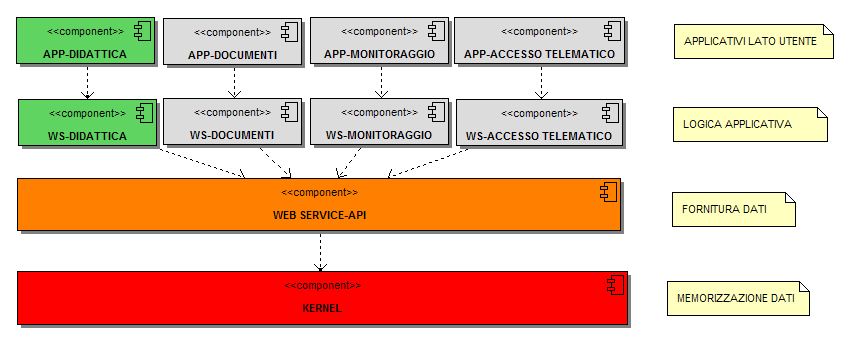
\includegraphics[width=10.5cm]{img/ArchitetturaGenerale.png}
\end{center}

\end{frame}

\begin{frame}
  \frametitle{Kernel}
  
 \begin{itemize}
\item componente che memorizza le informazioni della scuola e si assicura che siano coerenti e corrette
\item realizzata da Swell Systems
\end{itemize}

\end{frame}

\begin{frame}
\frametitle{Web Service-API}

\begin{itemize}
\item componente che permette di usufruire dei servizi del kernel esponendo un Web Service
\item progettata congiuntamente per preparare un terreno fertile allo sviluppo dei moduli previsti e per quelli futuri
\item realizzata da Swell Systems
\end{itemize}

\end{frame}

\begin{frame}
\frametitle{Web Service dei moduli}
\framesubtitle{WS-Didattica, WS-Documenti, WS-Monitoraggio, WS-Accesso telematico}

\begin{itemize}
\item componenti che implementano la logica del prodotto
\item anche questi espongono un Web Service
\item parte di queste realizzate da Egoless Group
\end{itemize}

\end{frame}

\begin{frame}
\frametitle{Applicazioni desktop}
\framesubtitle{APP-Didattica, APP-Documenti, APP-Monitoraggio, APP-Accesso telematico}

\begin{itemize}
\item programmi che permettono all'utente di interagire con il sistema
\item per svolgere il loro lavoro consumano i Web Service dei moduli
\item parte di questi realizzati da Egoless Group
\end{itemize}

\end{frame}

\subsection{WS-Didattica e APP-Didattica}

\begin{frame}
\frametitle{Cosa realizziamo nella prima iterazione}

\begin{itemize}
\item solo le funzionalità fondamentali del modulo didattica
\begin{itemize}
\item per poter acquisire conoscenze consolidate delle tecnologie
\item evitare la propagazione contemporanea di errori e disfunzioni ad altri moduli con implementazioni simili
\item produrre in tempo un qualcosa di funzionante e stabile
\item ...in definitiva \alert{evitare embrionali debolezze strutturali!}
\end{itemize}
%\end{itemize}

\item più un prototipo che un prodotto
\end{itemize}
\end{frame}

\begin{frame}
\frametitle{Funzionalità contemplate nella prima iterazione}

\begin{itemize}
\item gestione di studenti e professori
\item per gli studenti gestione di assenze e votazioni
\item il tutto senza autenticazione
\end{itemize}

\end{frame}

\begin{frame}
\frametitle{APP-Didattica}

\begin{itemize}
\item permette all'utente di svolgere le azioni di sua competenza
\item applicazione desktop-oriented
\begin{itemize}
\item il personale didattico è abituato a programmi come Word ed Excel
\item miglior supporto tecnologico per interfacce grafiche ricche ed intuitive (per esempio drag and drop)
\end{itemize}

\end{itemize}

\end{frame}

\begin{frame}
\frametitle{WS-Didattica}
\framesubtitle{Considerazioni progettuali}

\begin{itemize}
\item l'impiego di tecnologie che generano l'infrastruttura del Web Service a partire dal codice permette di progettare direttamente le classi
\item classi
\begin{itemize}
\item uso dell'id
\item distinzione tra classi semplici, complesse e per la ricerca
\end{itemize}

\item metodi del Web Service
\begin{itemize}
\item più o meno simili per classi semplici e complesse
\item attenzione alle quantità di dati trasferite
\end{itemize}


\end{itemize}

\end{frame}

\section{Evoluzione Piano di Qualifica}
\subsection{Tracciamento}

\begin{frame}
\frametitle{Cos'è il tracciamento}



\begin{itemize}
\item Garantisce qualità, limitando la creatività.
\begin{itemize}
\item Ogni prodotto intermedio deve essere sufficiente e necessario.
\end{itemize}
\item Applica ad ogni fase del ciclo di vita del prodotto software.
\begin{itemize}
\item Mantiene una mappatura degli ingressi nelle uscite di ogni fase.
\end{itemize}
\end{itemize}

\end{frame}

\begin{frame}
\frametitle{Quando si svolge il tracciamento}
\begin{center}
  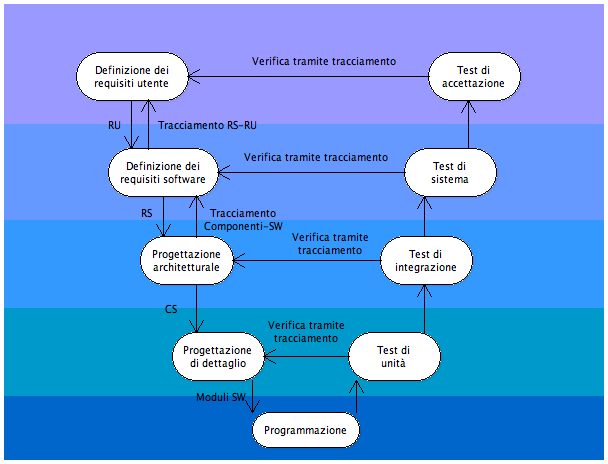
\includegraphics[width=10cm]{img/Vmodel.png}
\end{center}
\end{frame}

\begin{frame}
\frametitle{Come svolgiamo il tracciamento}

\begin{itemize}
\item Il tutto viene implementato:
	\begin{itemize}
		\item Assegnando identificatori univoci ad ogni entità.
		\item Compilando le matrici di tracciamento.
	\end{itemize}
\end{itemize}

\end{frame}

\subsection{Metodi verifica}

\begin{frame}
\frametitle{Metodi di verifica}

\begin{itemize}
\item abbiamo individuato in maniera più precisa gli strumenti per la verifica
\item codifica
\begin{itemize}
\item analisi statica
\item analisi dinamica
\end{itemize}
\item processi
\begin{itemize}
\item PDCA
\item metriche
\end{itemize}
\end{itemize}

\end{frame}

\section{Cosa abbiamo sbagliato finora}

\subsection*{Cosa abbiamo sbagliato finora}

\begin{frame}
\frametitle{Cosa abbiamo sbagliato finora}

\begin{itemize}
\item la pianificazione si è rivelata essere errata
\begin{itemize}
\item troppe ore per analisi e verifica
\item troppo poche per progettazione
\item la nostra intenzione è di recuperarle più avanti
\end{itemize}

\item ritardo nel mettere in opera l'ambiente di lavoro
\item gestione della collaborazione ancora un po' problematica
\end{itemize}

\end{frame}

\end{document}